% Options for packages loaded elsewhere
\PassOptionsToPackage{unicode}{hyperref}
\PassOptionsToPackage{hyphens}{url}
\PassOptionsToPackage{dvipsnames,svgnames,x11names}{xcolor}
%
\documentclass[
  letterpaper,
  DIV=11,
  numbers=noendperiod]{scrartcl}

\usepackage{amsmath,amssymb}
\usepackage{iftex}
\ifPDFTeX
  \usepackage[T1]{fontenc}
  \usepackage[utf8]{inputenc}
  \usepackage{textcomp} % provide euro and other symbols
\else % if luatex or xetex
  \usepackage{unicode-math}
  \defaultfontfeatures{Scale=MatchLowercase}
  \defaultfontfeatures[\rmfamily]{Ligatures=TeX,Scale=1}
\fi
\usepackage{lmodern}
\ifPDFTeX\else  
    % xetex/luatex font selection
\fi
% Use upquote if available, for straight quotes in verbatim environments
\IfFileExists{upquote.sty}{\usepackage{upquote}}{}
\IfFileExists{microtype.sty}{% use microtype if available
  \usepackage[]{microtype}
  \UseMicrotypeSet[protrusion]{basicmath} % disable protrusion for tt fonts
}{}
\makeatletter
\@ifundefined{KOMAClassName}{% if non-KOMA class
  \IfFileExists{parskip.sty}{%
    \usepackage{parskip}
  }{% else
    \setlength{\parindent}{0pt}
    \setlength{\parskip}{6pt plus 2pt minus 1pt}}
}{% if KOMA class
  \KOMAoptions{parskip=half}}
\makeatother
\usepackage{xcolor}
\setlength{\emergencystretch}{3em} % prevent overfull lines
\setcounter{secnumdepth}{5}
% Make \paragraph and \subparagraph free-standing
\ifx\paragraph\undefined\else
  \let\oldparagraph\paragraph
  \renewcommand{\paragraph}[1]{\oldparagraph{#1}\mbox{}}
\fi
\ifx\subparagraph\undefined\else
  \let\oldsubparagraph\subparagraph
  \renewcommand{\subparagraph}[1]{\oldsubparagraph{#1}\mbox{}}
\fi


\providecommand{\tightlist}{%
  \setlength{\itemsep}{0pt}\setlength{\parskip}{0pt}}\usepackage{longtable,booktabs,array}
\usepackage{calc} % for calculating minipage widths
% Correct order of tables after \paragraph or \subparagraph
\usepackage{etoolbox}
\makeatletter
\patchcmd\longtable{\par}{\if@noskipsec\mbox{}\fi\par}{}{}
\makeatother
% Allow footnotes in longtable head/foot
\IfFileExists{footnotehyper.sty}{\usepackage{footnotehyper}}{\usepackage{footnote}}
\makesavenoteenv{longtable}
\usepackage{graphicx}
\makeatletter
\def\maxwidth{\ifdim\Gin@nat@width>\linewidth\linewidth\else\Gin@nat@width\fi}
\def\maxheight{\ifdim\Gin@nat@height>\textheight\textheight\else\Gin@nat@height\fi}
\makeatother
% Scale images if necessary, so that they will not overflow the page
% margins by default, and it is still possible to overwrite the defaults
% using explicit options in \includegraphics[width, height, ...]{}
\setkeys{Gin}{width=\maxwidth,height=\maxheight,keepaspectratio}
% Set default figure placement to htbp
\makeatletter
\def\fps@figure{htbp}
\makeatother
% definitions for citeproc citations
\NewDocumentCommand\citeproctext{}{}
\NewDocumentCommand\citeproc{mm}{%
  \begingroup\def\citeproctext{#2}\cite{#1}\endgroup}
\makeatletter
 % allow citations to break across lines
 \let\@cite@ofmt\@firstofone
 % avoid brackets around text for \cite:
 \def\@biblabel#1{}
 \def\@cite#1#2{{#1\if@tempswa , #2\fi}}
\makeatother
\newlength{\cslhangindent}
\setlength{\cslhangindent}{1.5em}
\newlength{\csllabelwidth}
\setlength{\csllabelwidth}{3em}
\newenvironment{CSLReferences}[2] % #1 hanging-indent, #2 entry-spacing
 {\begin{list}{}{%
  \setlength{\itemindent}{0pt}
  \setlength{\leftmargin}{0pt}
  \setlength{\parsep}{0pt}
  % turn on hanging indent if param 1 is 1
  \ifodd #1
   \setlength{\leftmargin}{\cslhangindent}
   \setlength{\itemindent}{-1\cslhangindent}
  \fi
  % set entry spacing
  \setlength{\itemsep}{#2\baselineskip}}}
 {\end{list}}
\usepackage{calc}
\newcommand{\CSLBlock}[1]{\hfill\break\parbox[t]{\linewidth}{\strut\ignorespaces#1\strut}}
\newcommand{\CSLLeftMargin}[1]{\parbox[t]{\csllabelwidth}{\strut#1\strut}}
\newcommand{\CSLRightInline}[1]{\parbox[t]{\linewidth - \csllabelwidth}{\strut#1\strut}}
\newcommand{\CSLIndent}[1]{\hspace{\cslhangindent}#1}

\KOMAoption{captions}{tableheading}
\makeatletter
\@ifpackageloaded{caption}{}{\usepackage{caption}}
\AtBeginDocument{%
\ifdefined\contentsname
  \renewcommand*\contentsname{Table of contents}
\else
  \newcommand\contentsname{Table of contents}
\fi
\ifdefined\listfigurename
  \renewcommand*\listfigurename{List of Figures}
\else
  \newcommand\listfigurename{List of Figures}
\fi
\ifdefined\listtablename
  \renewcommand*\listtablename{List of Tables}
\else
  \newcommand\listtablename{List of Tables}
\fi
\ifdefined\figurename
  \renewcommand*\figurename{Figure}
\else
  \newcommand\figurename{Figure}
\fi
\ifdefined\tablename
  \renewcommand*\tablename{Table}
\else
  \newcommand\tablename{Table}
\fi
}
\@ifpackageloaded{float}{}{\usepackage{float}}
\floatstyle{ruled}
\@ifundefined{c@chapter}{\newfloat{codelisting}{h}{lop}}{\newfloat{codelisting}{h}{lop}[chapter]}
\floatname{codelisting}{Listing}
\newcommand*\listoflistings{\listof{codelisting}{List of Listings}}
\makeatother
\makeatletter
\makeatother
\makeatletter
\@ifpackageloaded{caption}{}{\usepackage{caption}}
\@ifpackageloaded{subcaption}{}{\usepackage{subcaption}}
\makeatother
\ifLuaTeX
  \usepackage{selnolig}  % disable illegal ligatures
\fi
\usepackage{bookmark}

\IfFileExists{xurl.sty}{\usepackage{xurl}}{} % add URL line breaks if available
\urlstyle{same} % disable monospaced font for URLs
\hypersetup{
  pdftitle={CN I: Olfactory nerve},
  pdfauthor={Nathaniel Giovanni Yomogida, SPT; Chloë Anne Kerstein, SPT},
  colorlinks=true,
  linkcolor={blue},
  filecolor={Maroon},
  citecolor={Blue},
  urlcolor={Blue},
  pdfcreator={LaTeX via pandoc}}

\title{CN I: Olfactory nerve}
\author{Nathaniel Yomogida, SPT \and Chloë Kerstein, SPT}
\date{}

\begin{document}
\maketitle

\renewcommand*\contentsname{Table of contents}
{
\hypersetup{linkcolor=}
\setcounter{tocdepth}{3}
\tableofcontents
}
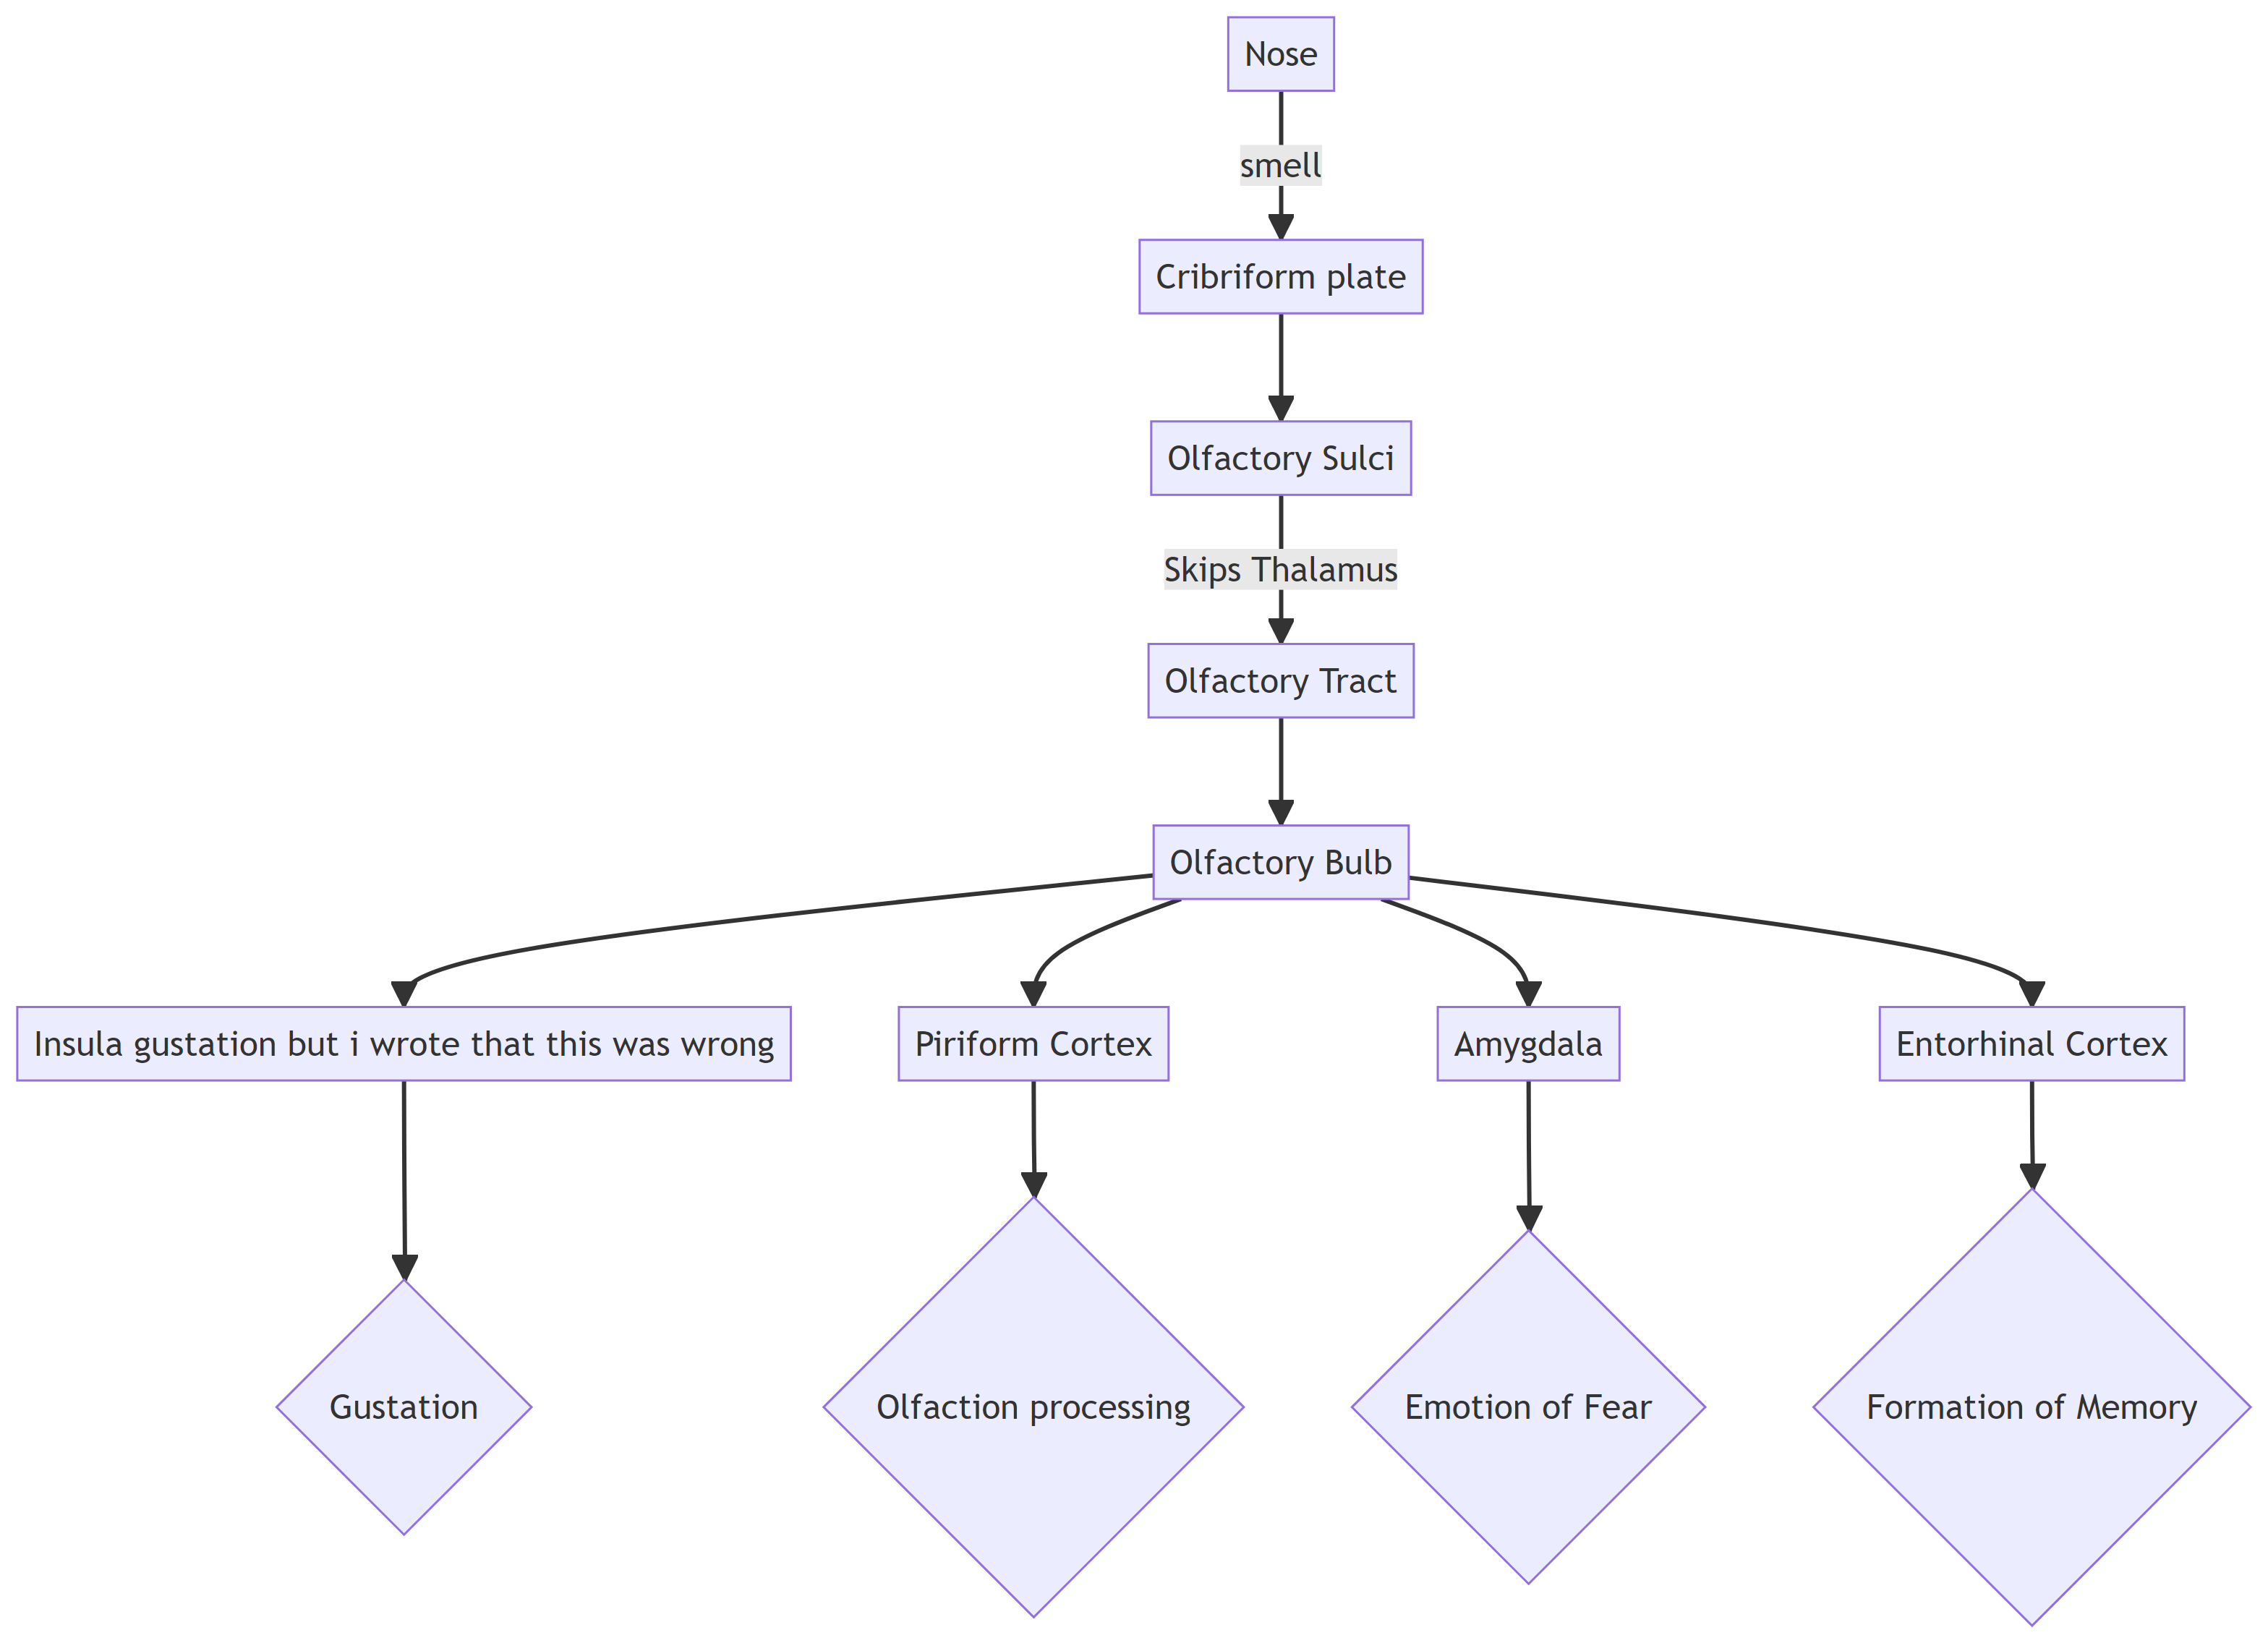
\includegraphics[width=10.93in,height=7.92in]{CN1_Olfactory_files/figure-latex/mermaid-figure-1.png}

\begin{figure}[H]

{\centering 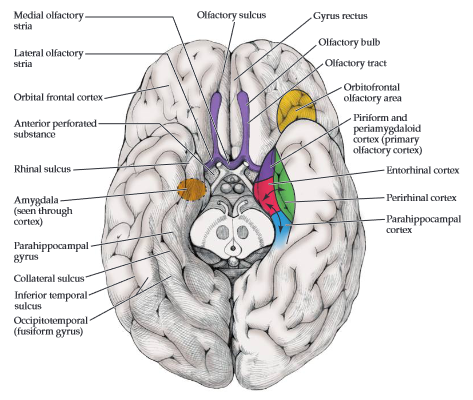
\includegraphics{../../../../Alchemy Archive/Neuro/Neuroanatomy/Cranial Nerves/images/fig18.6 central olfactory structures blumenfeldNeuroanatomyClinicalCases2022.png}

}

\caption{Central Olfactory Structures (from Blumenfield Figure
18.6\textsuperscript{\citeproc{ref-blumenfeldNeuroanatomyClinicalCases2022}{1}})}

\end{figure}%

\section{Pathway:}\label{pathway}

\subsection{First order neurons:}\label{first-order-neurons}

\begin{enumerate}
\def\labelenumi{\arabic{enumi}.}
\tightlist
\item
  Smell is detected by specialized chemoreceptors on bipolar primary
  sensory neurons found in the olfactory
  neuroepithelium\textsuperscript{\citeproc{ref-blumenfeldNeuroanatomyClinicalCases2022}{1}}
\item
  Olfactory nerve (made up of axons combined with other receptor cell
  axons)\textsuperscript{\citeproc{ref-blumenfeldNeuroanatomyClinicalCases2022}{1}}
\item
  Pass through Cribriform plate of Ethmoid
  bone\textsuperscript{\citeproc{ref-blumenfeldNeuroanatomyClinicalCases2022}{1}}
\item
  Terminate on the olfactory bulb (main relay station of olfactory
  pathway)\textsuperscript{\citeproc{ref-blumenfeldNeuroanatomyClinicalCases2022}{1}}
\end{enumerate}

\subsection{Second order neurons:}\label{second-order-neurons}

\begin{enumerate}
\def\labelenumi{\arabic{enumi}.}
\tightlist
\item
  Olfactory tract
\item
  Split: Medial \& Lateral striae

  \begin{enumerate}
  \def\labelenumii{\arabic{enumii}.}
  \tightlist
  \item
    Medial Stria: Projects to subcallosal gyrus
  \item
    Lateral Stria: continues on to Parahippocampal gyrus
  \end{enumerate}
\end{enumerate}

\section{Relevant Structures}\label{relevant-structures}

The olfactory nerve does not have peripheral ganglia

Olfactory cortex: no single structure - Piriform cortex: - Located:
Below lateral olfactory stria - Function: Olfactory processing -
\href{../../../../Alchemy\%20Archive/Neuro/Neuroanatomy/Limbic\%20System/amygdala.qmd}{Amygdala}:
- Located: Anterior to Temporal/Inferior horn of Lateral Ventricle -
Function: Emotion \& Fear - Entorhinal cortex: - Location: Anterior part
of Parahippocampal gyrus - Function: Formation of Memory

\section{Dysfunction}\label{dysfunction}

\begin{itemize}
\tightlist
\item
  \href{../../../../Alchemy\%20Archive/Neuro/Neuroanatomy/Neurophysiology/Neuro\%20Symptoms/anosmia.qmd}{Anosmia}
\end{itemize}

\phantomsection\label{refs}
\begin{CSLReferences}{0}{1}
\bibitem[\citeproctext]{ref-blumenfeldNeuroanatomyClinicalCases2022}
\CSLLeftMargin{1. }%
\CSLRightInline{Blumenfeld H. \emph{Neuroanatomy Through Clinical
Cases}. 3rd ed. {Oxford university press}; 2022.}

\end{CSLReferences}



\end{document}
